\documentclass[12pt,a4paper]{report}

% =========================================================
% Recruitment Management System Report
% Compile suggestion: pdfLaTeX or XeLaTeX on Overleaf.
% The first pages include the original Project 06 PDF as required.
% =========================================================

\usepackage[utf8]{inputenc}
\usepackage[T1]{fontenc}
\usepackage[english]{babel}
\usepackage{geometry}
\usepackage{setspace}
\usepackage{graphicx}
\usepackage{pdfpages}
\usepackage{booktabs}
\usepackage{longtable}
\usepackage{array}
\usepackage{enumitem}
\usepackage{float}
\usepackage{xcolor}
\usepackage{hyperref}
\usepackage{listings}
\usepackage{caption}
\usepackage{tikz}
\usetikzlibrary{positioning,arrows.meta}

\geometry{
  left=3cm,
  right=2.5cm,
  top=2.5cm,
  bottom=2.5cm
}

\onehalfspacing
\setlength{\parindent}{1.2cm}
\setlength{\parskip}{0.25em}
\setlength{\emergencystretch}{2em}
\renewcommand{\arraystretch}{1.25}
\newcolumntype{L}[1]{>{\raggedright\arraybackslash}p{#1}}

\hypersetup{
  colorlinks=true,
  linkcolor=blue!60!black,
  urlcolor=blue!60!black,
  citecolor=blue!60!black
}

\definecolor{codegray}{RGB}{245,247,250}
\definecolor{codeborder}{RGB}{220,226,235}
\definecolor{codered}{RGB}{170,40,40}
\definecolor{codeblue}{RGB}{20,80,160}

\lstdefinestyle{projectcode}{
  backgroundcolor=\color{codegray},
  basicstyle=\ttfamily\small,
  breaklines=true,
  frame=single,
  rulecolor=\color{codeborder},
  keywordstyle=\color{codeblue}\bfseries,
  commentstyle=\color{gray},
  stringstyle=\color{codered},
  showstringspaces=false,
  columns=fullflexible
}
\lstset{style=projectcode}

\newcommand{\projectname}{Recruitment Management System}
\newcommand{\studentname}{\textit{Student name}}
\newcommand{\studentid}{\textit{Student ID}}
\newcommand{\classname}{\textit{Class}}
\newcommand{\teachername}{\textit{Instructor}}
\newcommand{\githuburl}{\textit{GitHub repository link}}
\newcommand{\youtubeurl}{\textit{YouTube demonstration link}}
\newcommand{\codebreak}[1]{\begin{tabular}[t]{@{}l@{}}#1\end{tabular}}

\begin{document}

% =========================================================
% Required first pages: attach the original Project 06 PDF.
% If compiling this file from the report/ directory, ../6.pdf works.
% If compiling from the project root, 6.pdf works.
% =========================================================
\IfFileExists{../6.pdf}{
  \includepdf[pages=-,pagecommand={}]{../6.pdf}
}{
  \IfFileExists{6.pdf}{
    \includepdf[pages=-,pagecommand={}]{6.pdf}
  }{
    \begin{center}
      \Large\textbf{Project 06 requirement PDF should be attached here.}
    \end{center}
    \clearpage
  }
}

\begin{titlepage}
  \centering
  {\Large National Economics University\par}
  {\Large College of Technology\par}
  {\Large DATCOM Lab\par}
  \vspace{2.5cm}
  {\huge\bfseries PROJECT REPORT\par}
  \vspace{0.8cm}
  {\LARGE\bfseries \projectname\par}
  \vspace{1.5cm}
  \begin{tabular}{rl}
    Student: & \studentname \\
    Student ID: & \studentid \\
    Class: & \classname \\
    Instructor: & \teachername \\
    DBMS: & MySQL \\
    Programming language: & Python, TypeScript \\
  \end{tabular}
  \vfill
  {\large Hanoi, \the\year\par}
\end{titlepage}

\pagenumbering{roman}

\chapter*{Abstract}
\addcontentsline{toc}{chapter}{Abstract}

This report presents the design and implementation of a \projectname{} developed for Project 06. The system supports the main operations of a digital recruitment process, including candidate management, employer management, job posting, job application tracking, interview scheduling, interview result recording, reporting, and administrative control. The database is implemented in MySQL and contains relational tables, primary and foreign key constraints, indexes, views, stored procedures, user-defined functions, and triggers. The application layer is implemented with a FastAPI backend and a Next.js frontend. The system is deployed with MySQL on Railway, the backend API on Render, and the frontend on Vercel.

The report follows an undergraduate academic structure. It begins with requirement analysis, then describes the database design, advanced database objects, backend and frontend implementation, security mechanisms, cloud deployment, testing, and future improvement directions. The system also extends the basic project requirement by adding JWT authentication, role-based access control, ownership checks, audit logging, admin features, and deployment-ready configuration.

\noindent\textbf{Keywords:} recruitment management, MySQL, FastAPI, Next.js, database design, stored procedure, trigger, JWT, RBAC.

\tableofcontents
\listoffigures
\listoftables
\clearpage
\pagenumbering{arabic}

\chapter{Introduction}

\section{Project Background}

Recruitment is a data-intensive process that requires employers to publish job positions, candidates to submit applications, recruiters to track application status, and interviewers to evaluate candidates. If these operations are handled manually, the process can become slow, inconsistent, and difficult to audit. A database-driven recruitment management system provides a structured way to store recruitment data, enforce business rules, and support decision-making through reports.

The Project 06 requirement specifies a recruitment management system using MySQL as the database management system and Python as the main programming language. The required scope includes candidates, job positions, applications, interviews, employers, reports, database design, advanced database objects, security, administration, and a working Python application.

\section{Objectives}

The main objective of this project is to develop a recruitment management system that can manage the end-to-end workflow from job posting to interview result recording. The system is designed to satisfy both database requirements and application requirements.

The detailed objectives are:

\begin{itemize}[leftmargin=1.5cm]
  \item Design a normalized relational database for recruitment data.
  \item Implement constraints, indexes, views, procedures, functions, and triggers in MySQL.
  \item Build a backend API that exposes recruitment operations through REST endpoints.
  \item Build a modern frontend interface for candidates, employers, and administrators.
  \item Add authentication, authorization, ownership checks, and audit logs.
  \item Deploy the database, backend, and frontend to cloud platforms.
  \item Provide documentation, source code, and demonstration artifacts.
\end{itemize}

\section{Project Scope}

The system includes three main groups of users: candidates, employers, and administrators. Candidates can view job details, submit applications, upload or provide resumes, and track their application history. Employers can create jobs, view applications for their own jobs, schedule interviews, record interview results, and manage application statuses. Administrators can monitor the whole system, approve or deactivate employer accounts, inspect suspicious data, reset accounts, and review audit logs.

The implementation also includes deployment support through Railway, Render, and Vercel. Railway hosts the MySQL database, Render hosts the FastAPI backend, and Vercel hosts the Next.js frontend.

\chapter{Requirement Analysis}

\section{Functional Requirements}

Table \ref{tab:functional-requirements} summarizes the major functional requirements derived from Project 06 and the implemented extensions.

\begin{longtable}{L{0.28\textwidth}L{0.62\textwidth}}
\caption{Functional requirements of the system}
\label{tab:functional-requirements}\\
\toprule
\textbf{Module} & \textbf{Required functions} \\
\midrule
\endfirsthead
\toprule
\textbf{Module} & \textbf{Required functions} \\
\midrule
\endhead
Candidate management & Store candidate profile information such as full name, date of birth, phone number, account reference, resume information, and application history. \\
Employer management & Store employer profile information such as company name, contact number, address, account reference, approval status, and activation status. \\
Job posting & Allow employers to create, update, close, and view job positions. Each job is owned by one employer. \\
Application tracking & Allow candidates to apply for jobs and allow employers to track applications for their own job positions. \\
Interview scheduling & Allow employers to schedule interviews for applications, including interview time, location or meeting link, and notes. \\
Interview result recording & Allow employers to record interview result, score, and notes. Database triggers update application status after interview results are recorded. \\
Reporting & Provide dashboard metrics such as total users, jobs, applications, interviews, and monthly pass rate. \\
Administration & Allow administrators to view all major entities, approve or deactivate employers, disable accounts, reset passwords, inspect suspicious data, and review audit logs. \\
Authentication and authorization & Authenticate users by email and password, issue JWT tokens, enforce role-based permissions, and prevent users from accessing resources they do not own. \\
\bottomrule
\end{longtable}

\section{Non-functional Requirements}

The system is expected to satisfy the following non-functional requirements:

\begin{itemize}[leftmargin=1.5cm]
  \item \textbf{Data integrity:} primary keys, foreign keys, unique constraints, and check constraints must prevent invalid data.
  \item \textbf{Security:} passwords must be stored as hashes, not plain text. Backend authorization must be enforced based on JWT and user roles.
  \item \textbf{Maintainability:} backend functions, CRUD operations, database scripts, and frontend components should be organized by responsibility.
  \item \textbf{Usability:} the frontend should provide clear navigation for candidates, employers, and administrators.
  \item \textbf{Deployability:} the system should run locally and on cloud platforms with environment variables.
  \item \textbf{Auditability:} important operations should be written to an audit table for later inspection.
\end{itemize}

\section{User Roles}

The system uses four practical roles. The \texttt{Admin} role manages system-wide data. The \texttt{Employer} role manages company-owned jobs and applications. The \texttt{Candidate} role applies for jobs and manages candidate information. The legacy project description also mentions HR and interviewers; in the implemented system, these responsibilities are represented mainly through employer-side functions and can be separated further in future work.

\chapter{Database Design}

\section{Entity Model}

The system uses eight main entities: \texttt{Accounts}, \texttt{Employers}, \texttt{Candidates}, \texttt{JobPositions}, \texttt{Applications}, \texttt{Interviews}, \texttt{AuditLogs}, and \texttt{Notifications}. \texttt{Accounts} stores authentication and role information. \texttt{Employers} and \texttt{Candidates} store business profile information associated with accounts. \texttt{JobPositions} represents published jobs. \texttt{Applications} connects candidates to job positions. \texttt{Interviews} stores interview schedule and result data. \texttt{AuditLogs} records important actions. \texttt{Notifications} stores messages created by actions such as scheduling interviews or recording results.

\begin{figure}[H]
\centering
\resizebox{0.96\textwidth}{!}{%
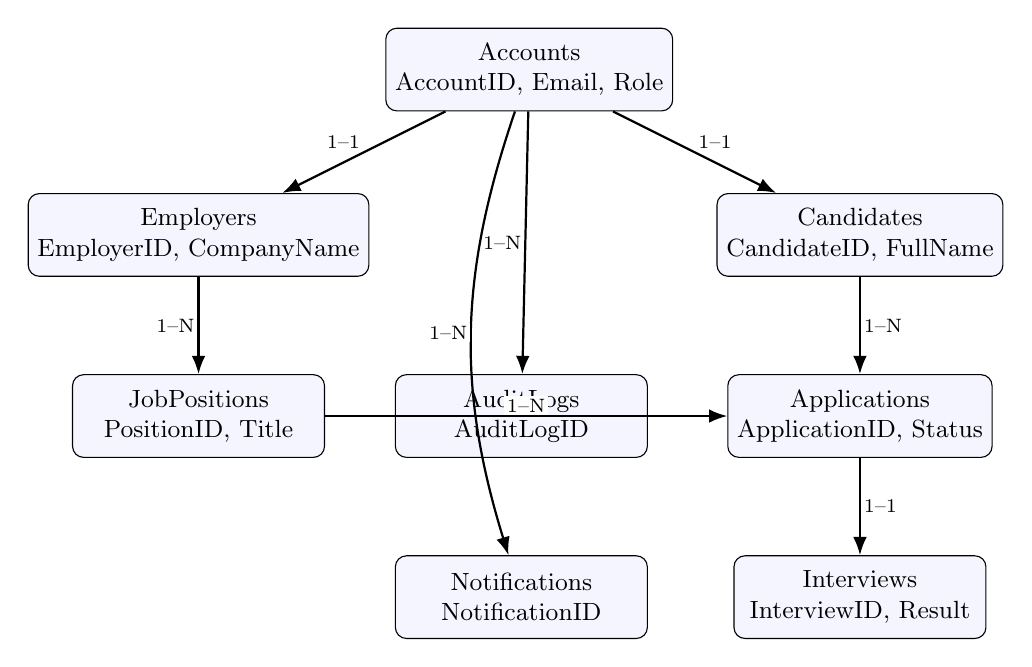
\begin{tikzpicture}[
  entity/.style={
    draw,
    rounded corners,
    align=center,
    minimum width=3.2cm,
    minimum height=1.05cm,
    fill=blue!4,
    font=\small
  },
  rel/.style={-Latex, thick},
  labelstyle/.style={font=\scriptsize, fill=white, inner sep=1pt}
]
  \node[entity] (accounts) at (0,0) {Accounts\\AccountID, Email, Role};
  \node[entity] (employers) at (-4.2,-2.1) {Employers\\EmployerID, CompanyName};
  \node[entity] (candidates) at (4.2,-2.1) {Candidates\\CandidateID, FullName};
  \node[entity] (jobs) at (-4.2,-4.4) {JobPositions\\PositionID, Title};
  \node[entity] (applications) at (4.2,-4.4) {Applications\\ApplicationID, Status};
  \node[entity] (interviews) at (4.2,-6.7) {Interviews\\InterviewID, Result};
  \node[entity] (audit) at (-0.1,-4.4) {AuditLogs\\AuditLogID};
  \node[entity] (notifications) at (-0.1,-6.7) {Notifications\\NotificationID};

  \draw[rel] (accounts) -- node[labelstyle, above left]{1--1} (employers);
  \draw[rel] (accounts) -- node[labelstyle, above right]{1--1} (candidates);
  \draw[rel] (employers) -- node[labelstyle, left]{1--N} (jobs);
  \draw[rel] (candidates) -- node[labelstyle, right]{1--N} (applications);
  \draw[rel] (jobs) -- node[labelstyle, above]{1--N} (applications);
  \draw[rel] (applications) -- node[labelstyle, right]{1--1} (interviews);
  \draw[rel] (accounts) -- node[labelstyle, left]{1--N} (audit);
  \draw[rel] (accounts) to[bend right=18] node[labelstyle, left]{1--N} (notifications);
\end{tikzpicture}%
}
\caption{Conceptual ER model of the recruitment management system}
\label{fig:er-model}
\end{figure}

The diagram in Figure \ref{fig:er-model} is intentionally presented at a conceptual level. The physical schema contains additional attributes such as dates, status values, contact details, password hash, timestamps, and foreign key references. The one-to-one relation from \texttt{Accounts} to \texttt{Employers} or \texttt{Candidates} represents profile ownership. The one-to-many relation from \texttt{Employers} to \texttt{JobPositions} enforces employer ownership of job postings.

\section{Relational Schema}

Table \ref{tab:relational-schema} describes the main tables in the relational schema.

\begin{longtable}{L{0.24\textwidth}L{0.66\textwidth}}
\caption{Main relational tables}
\label{tab:relational-schema}\\
\toprule
\textbf{Table} & \textbf{Purpose and important attributes} \\
\midrule
\endfirsthead
\toprule
\textbf{Table} & \textbf{Purpose and important attributes} \\
\midrule
\endhead
\texttt{Accounts} & Stores login identity, email, password hash, role, activation status, and timestamps. It is the root table for authentication and authorization. \\
\texttt{Employers} & Stores company profile data such as company name, contact number, address, account reference, approval status, and activation status. \\
\texttt{Candidates} & Stores candidate profile data such as full name, date of birth, phone number, resume URL or uploaded CV reference, and account reference. \\
\texttt{JobPositions} & Stores job posting data such as employer ID, title, description, requirements, salary, posted date, and status. \\
\texttt{Applications} & Stores candidate applications for job positions, including candidate ID, position ID, status, applied date, and related metadata. \\
\texttt{Interviews} & Stores interview schedule and result data, including application ID, interview time, location or meeting link, result, score, and notes. \\
\texttt{AuditLogs} & Stores important actions such as creating jobs, changing application status, recording interview results, account changes, and admin actions. \\
\texttt{Notifications} & Stores system notifications sent to users when interviews are scheduled or results are recorded. \\
\bottomrule
\end{longtable}

\section{Constraints}

The database uses constraints to protect data correctness at the storage level. This is important because the backend, the frontend, and administrative scripts may all interact with the same data. If integrity rules are only implemented in the application layer, invalid data can still be inserted by another client or by a direct SQL import. For this reason, the project places the most important business rules in the MySQL schema.

\begin{longtable}{L{0.27\textwidth}L{0.63\textwidth}}
\caption{Main database constraints and their purposes}
\label{tab:constraints}\\
\toprule
\textbf{Constraint group} & \textbf{Purpose in the system} \\
\midrule
\endfirsthead
\toprule
\textbf{Constraint group} & \textbf{Purpose in the system} \\
\midrule
\endhead
\codebreak{Primary key\\constraints} & \texttt{AccountID}, \texttt{EmployerID}, \texttt{CandidateID}, \texttt{PositionID}, \texttt{ApplicationID}, \texttt{InterviewID}, \texttt{AuditLogID}, and \texttt{NotificationID} uniquely identify each record. They are also used as stable references in API responses and foreign-key relationships. \\
\codebreak{\texttt{uq\_accounts}\\\texttt{\_email}} & Ensures that every login email is unique. This prevents two accounts from sharing the same credential identity and allows the backend to authenticate users by email safely. \\
\codebreak{\texttt{uq\_employers}\\\texttt{\_account}\\and\\\texttt{uq\_candidates}\\\texttt{\_account}} & Ensure that one account can be linked to only one employer profile or one candidate profile. This keeps authentication data separated from business profile data while preserving a one-to-one relationship. \\
\codebreak{\texttt{uq\_applications}\\\texttt{\_candidate}\\\texttt{\_position}} & Prevents the same candidate from applying to the same job position more than once. This supports application tracking and avoids duplicate rows in employer dashboards. \\
\codebreak{\texttt{uq\_interviews}\\\texttt{\_application}} & Ensures that each application has at most one interview record in the current design. This makes interview scheduling and result recording easier to manage. \\
\codebreak{Foreign keys\\from profiles\\to accounts} & \texttt{fk\_employers\_account} and \texttt{fk\_candidates\_account} connect business profiles to login accounts. They use cascading update and delete behavior so profile records stay synchronized with their account records. \\
\codebreak{Foreign keys\\for recruitment\\workflow} & The foreign keys on employer, candidate, position, and application references enforce the workflow from employer to job, candidate to application, job to application, and application to interview. \\
\codebreak{Foreign keys\\for administration} & The audit-log actor reference keeps audit records linked to the actor account when possible. If an account is deleted, the audit row can remain with a null actor. The notification account reference links notifications to the receiving user. \\
Status enumerations & MySQL \texttt{ENUM} columns restrict values such as account role, account status, employer approval status, job status, application status, and interview result. This prevents invalid states such as an unknown job status or an unsupported user role. \\
\codebreak{\texttt{chk\_interviews}\\\texttt{\_score}} & Restricts interview scores to the range from 0 to 10 when a score is provided. This protects reporting functions such as average interview score and pass-rate analysis. \\
\bottomrule
\end{longtable}

These constraints reduce repeated validation logic in the application layer and make the database a reliable source of truth. For example, the backend still checks whether a job is open before submitting an application, but the duplicate-application unique constraint provides a final database-level guarantee against duplicate applications.

\section{Indexes}

Indexes are added to columns that are frequently used in filtering, joining, duplicate checking, authentication, and reporting. The schema contains three explicit secondary indexes and several implicit indexes created by primary keys and unique constraints. In MySQL, primary keys and unique constraints are indexed automatically, so they also contribute to query performance.

\begin{longtable}{L{0.25\textwidth}L{0.26\textwidth}L{0.39\textwidth}}
\caption{Indexes and their effects}
\label{tab:indexes}\\
\toprule
\textbf{Index} & \textbf{Column or table} & \textbf{Effect} \\
\midrule
\endfirsthead
\toprule
\textbf{Index} & \textbf{Column or table} & \textbf{Effect} \\
\midrule
\endhead
Primary key indexes & All main entity ID columns & Speed up joins between entities, for example joining \texttt{Applications} to \texttt{Candidates}, \texttt{JobPositions}, and \texttt{Interviews}. They also make record lookup by ID efficient for REST API endpoints. \\
\codebreak{\texttt{uq\_accounts}\\\texttt{\_email}} & \codebreak{\texttt{Accounts}\\\texttt{.Email}} & Improves login lookup because authentication starts by finding an account by email. It also prevents duplicate login identities. \\
\codebreak{\texttt{uq\_applications}\\\texttt{\_candidate}\\\texttt{\_position}} & \codebreak{\texttt{Applications}\\\texttt{(CandidateID,}\\\texttt{PositionID)}} & Speeds up duplicate-application checks and supports candidate history queries filtered by candidate and job. \\
\codebreak{\texttt{uq\_interviews}\\\texttt{\_application}} & \codebreak{\texttt{Interviews}\\\texttt{.ApplicationID}} & Speeds up interview lookup when scheduling or recording a result for a specific application. It also enforces the one-interview-per-application rule. \\
\codebreak{\texttt{idx\_jobpositions}\\\texttt{\_status}} & \codebreak{\texttt{JobPositions}\\\texttt{.Status}} & Speeds up public job listing queries such as selecting only \texttt{Open} jobs. It also helps admin and employer screens filter open and closed jobs. \\
\codebreak{\texttt{idx\_applications}\\\texttt{\_status}} & \codebreak{\texttt{Applications}\\\texttt{.Status}} & Speeds up employer dashboards that filter applications by states such as \texttt{Pending}, \texttt{Reviewed}, \texttt{Interviewing}, \texttt{Rejected}, or \texttt{Accepted}. \\
\codebreak{\texttt{idx\_interviews}\\\texttt{\_date}} & \codebreak{\texttt{Interviews}\\\texttt{.InterviewDate}} & Speeds up calendar-style queries, upcoming interview lists, monthly reports, and date-based administrative monitoring. \\
Foreign-key supporting indexes & Child-side relationship columns & Support joins and referential checks for common paths such as employer to jobs, job to applications, candidate to applications, and application to interview. \\
\bottomrule
\end{longtable}

These indexes are selected based on the expected access patterns of the system. Candidate pages require quick lookup of open jobs and candidate applications. Employer pages require filtering applications by status and joining applications to jobs and interviews. Admin dashboards require aggregate queries over jobs, applications, and interviews. Therefore, the indexes support both operational screens and reporting screens.

\chapter{Advanced Database Objects}

\section{Views}

Views provide reusable query definitions for reporting and frontend dashboards. They reduce duplication in application code and make business-level data easier to consume.

\begin{longtable}{L{0.30\textwidth}L{0.60\textwidth}}
\caption{Views and their purposes}
\label{tab:views}\\
\toprule
\textbf{View} & \textbf{Purpose} \\
\midrule
\endfirsthead
\toprule
\textbf{View} & \textbf{Purpose} \\
\midrule
\endhead
\codebreak{\texttt{vw\_open}\\\texttt{\_job}\\\texttt{\_positions}} & Lists active job positions visible to candidates. \\
\codebreak{\texttt{vw\_candidate}\\\texttt{\_application}\\\texttt{\_tracker}} & Shows candidate application status with job and employer information. \\
\codebreak{\texttt{vw\_shortlisted}\\\texttt{\_candidates}} & Lists candidates with interview or reviewed status. \\
\codebreak{\texttt{vw\_job}\\\texttt{\_application}\\\texttt{\_summary}} & Summarizes applications per job position. \\
\codebreak{\texttt{vw\_interview}\\\texttt{\_results}} & Combines interview data with application, candidate, and job information. \\
\codebreak{\texttt{vw\_employer}\\\texttt{\_dashboard}\\\texttt{\_metrics}} & Provides employer-level metrics for dashboard cards. \\
\codebreak{\texttt{vw\_admin}\\\texttt{\_system}\\\texttt{\_metrics}} & Provides system-wide metrics for the administrator dashboard. \\
\bottomrule
\end{longtable}

\section{Stored Procedures}

Stored procedures are used for important workflows that should be executed consistently. They place business validation close to the data and reduce the risk of inconsistent updates from different application screens. The backend calls these procedures through SQLAlchemy or direct SQL execution when it performs recruitment operations.

\begin{longtable}{L{0.28\textwidth}L{0.62\textwidth}}
\caption{Stored procedures and their purposes}
\label{tab:procedures}\\
\toprule
\textbf{Stored procedure} & \textbf{Validation and effect} \\
\midrule
\endfirsthead
\toprule
\textbf{Stored procedure} & \textbf{Validation and effect} \\
\midrule
\endhead
\codebreak{\texttt{sp\_create}\\\texttt{\_job\_position}} & Validates that the employer exists, the job title is not empty, the job description is not empty, and the status is either \texttt{Open} or \texttt{Closed}. If validation passes, it inserts a new job position and returns the new \texttt{PositionID}. \\
\codebreak{\texttt{sp\_update}\\\texttt{\_job\_status}} & Validates that the job position exists and that the new status is valid. It updates the job status, which is used when an employer closes or reopens a job. \\
\codebreak{\texttt{sp\_submit}\\\texttt{\_application}} & Validates that the candidate exists, the job exists, the job is currently \texttt{Open}, and the candidate has not already applied to the same job. If validation passes, it creates a new application with \texttt{Pending} status. \\
\codebreak{\texttt{sp\_schedule}\\\texttt{\_interview}} & Validates that the application exists, no interview has already been scheduled for that application, the interview date is provided, and the interview date is later than the application date. It then creates an interview with \texttt{Pending} result. \\
\codebreak{\texttt{sp\_record}\\\texttt{\_interview}\\\texttt{\_result}} & Validates that an interview exists for the application, the result is one of \texttt{Pending}, \texttt{Pass}, or \texttt{Fail}, and final results have a score between 0 and 10. It updates the interview result, score, and notes. The interview trigger then updates the related application status. \\
\bottomrule
\end{longtable}

\begin{lstlisting}[language=SQL,caption={Example procedure style for recording an interview result}]
CALL sp_record_interview_result(
  p_application_id,
  p_result,
  p_score,
  p_notes
);
\end{lstlisting}

\section{User-defined Functions}

User-defined functions support reusable calculations. They are especially useful for dashboards because they express business metrics close to the data and can be reused by views, reports, or backend queries.

\begin{longtable}{L{0.28\textwidth}L{0.62\textwidth}}
\caption{User-defined functions and their purposes}
\label{tab:functions}\\
\toprule
\textbf{Function} & \textbf{Returned value and use} \\
\midrule
\endfirsthead
\toprule
\textbf{Function} & \textbf{Returned value and use} \\
\midrule
\endhead
\codebreak{\texttt{fn\_application\_count}\\\texttt{\_by\_position}\\\texttt{(p\_position\_id)}} & Returns the number of applications for a given job position. It is useful for employer job summaries and job-level reporting. \\
\codebreak{\texttt{fn\_candidate}\\\texttt{\_application\_count}\\\texttt{(p\_candidate\_id)}} & Returns the number of applications submitted by a candidate. It supports candidate activity reports and candidate profile pages. \\
\codebreak{\texttt{fn\_employer}\\\texttt{\_pass\_rate}\\\texttt{(p\_employer\_id)}} & Calculates the percentage of interviews with \texttt{Pass} result for a specific employer. If the employer has no interviews, it returns 0.00. This function supports dashboard pass-rate metrics. \\
\codebreak{\texttt{fn\_average}\\\texttt{\_interview\_score}\\\texttt{(p\_employer\_id)}} & Returns the average interview score for an employer, excluding null scores. It supports employer performance analysis and interview quality reporting. \\
\bottomrule
\end{longtable}

For example, the employer pass-rate function joins \texttt{Interviews}, \texttt{Applications}, and \texttt{JobPositions} to ensure that the calculation is limited to jobs owned by the selected employer. This prevents pass-rate data from mixing results from different companies.

\section{Triggers}

Triggers automate dependent updates that must happen whenever interview data changes. In this project, triggers keep \texttt{Applications.Status} synchronized with \texttt{Interviews.Result}. This prevents the backend or frontend from forgetting to update the application after an interview is scheduled or completed.

\begin{longtable}{L{0.28\textwidth}L{0.62\textwidth}}
\caption{Triggers and their effects}
\label{tab:triggers}\\
\toprule
\textbf{Trigger} & \textbf{Effect} \\
\midrule
\endfirsthead
\toprule
\textbf{Trigger} & \textbf{Effect} \\
\midrule
\endhead
\codebreak{\texttt{trg\_interviews}\\\texttt{\_after\_insert}\\\texttt{\_status}} & Runs after a new interview row is inserted. If the new interview result is \texttt{Pass}, the related application becomes \texttt{Accepted}. If the result is \texttt{Fail}, the application becomes \texttt{Rejected}. Otherwise, the application becomes \texttt{Interviewing}. \\
\codebreak{\texttt{trg\_interviews}\\\texttt{\_after\_update}\\\texttt{\_status}} & Runs after an existing interview row is updated. It applies the same mapping from interview result to application status, so changing a result from \texttt{Pending} to \texttt{Pass} or \texttt{Fail} automatically updates the application. \\
\bottomrule
\end{longtable}

The trigger logic creates a clear dependency rule: interview state controls application state after the interview stage begins. This improves consistency for employer dashboards, candidate application tracking, and administrative reports.

\chapter{Application Design and Implementation}

\section{Overall Architecture}

The system follows a three-layer architecture. The database layer is MySQL hosted on Railway. The backend layer is a FastAPI application hosted on Render and connected to MySQL through SQLAlchemy and mysql-connector-python. The frontend layer is a Next.js application hosted on Vercel and communicates with the backend through REST APIs using JWT authentication.

\begin{figure}[H]
\centering
\resizebox{0.92\textwidth}{!}{%
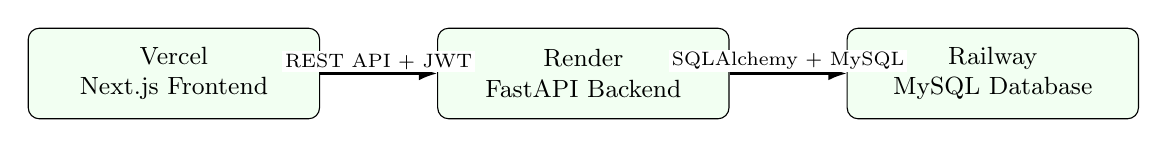
\begin{tikzpicture}[
  box/.style={
    draw,
    rounded corners,
    align=center,
    minimum width=3.7cm,
    minimum height=1.15cm,
    fill=green!5,
    font=\small
  },
  arrow/.style={-Latex, thick},
  lab/.style={font=\scriptsize, fill=white, inner sep=1pt}
]
  \node[box] (frontend) at (0,0) {Vercel\\Next.js Frontend};
  \node[box] (backend) at (5.2,0) {Render\\FastAPI Backend};
  \node[box] (database) at (10.4,0) {Railway\\MySQL Database};

  \draw[arrow] (frontend) -- node[lab, above]{REST API + JWT} (backend);
  \draw[arrow] (backend) -- node[lab, above]{SQLAlchemy + MySQL} (database);
\end{tikzpicture}%
}
\caption{Cloud deployment architecture}
\label{fig:deployment-architecture}
\end{figure}

Figure \ref{fig:deployment-architecture} shows the final deployment architecture. The frontend does not connect directly to the database. All data access goes through the backend API so that authentication, authorization, ownership checks, validation, and audit logging can be enforced in one place.

\section{Database Layer and Railway Hosting}

The database layer is the foundation of the system because it stores all persistent recruitment data and enforces the main data-integrity rules. The project uses MySQL because it supports relational modeling, foreign keys, views, stored procedures, functions, triggers, indexes, and transaction-based updates. These features match the requirements of Project 06 and allow the system to place important business rules close to the data.

In local development, the database can be created by running the SQL scripts against a local MySQL server. In cloud deployment, the same schema is imported into a Railway MySQL service. Railway provides a managed MySQL instance with persistent storage, connection variables, public TCP proxy access, and backup support. The backend service on Render connects to Railway through environment variables instead of hard-coded credentials.

\begin{longtable}{L{0.28\textwidth}L{0.62\textwidth}}
\caption{Database import scripts and their purposes}
\label{tab:database-scripts}\\
\toprule
\textbf{Script} & \textbf{Purpose} \\
\midrule
\endfirsthead
\toprule
\textbf{Script} & \textbf{Purpose} \\
\midrule
\endhead
\codebreak{\texttt{cloud\_00}\\\texttt{\_reset.sql}} & Optional reset script used when the deployed Railway database must be recreated from the beginning. It disables foreign-key checks temporarily and drops existing project tables. \\
\codebreak{\texttt{cloud\_01}\\\texttt{\_schema.sql}} & Creates the main tables, primary keys, foreign keys, unique constraints, check constraints, enum fields, and explicit indexes. \\
\codebreak{\texttt{cloud\_02}\\\texttt{\_views.sql}} & Creates reporting and dashboard views used by candidate, employer, and admin screens. \\
\codebreak{\texttt{cloud\_03}\\\texttt{\_routines.sql}} & Creates stored procedures and user-defined functions for job creation, application submission, interview scheduling, interview result recording, and dashboard metrics. \\
\codebreak{\texttt{cloud\_04}\\\texttt{\_triggers.sql}} & Creates interview triggers that synchronize application status with interview result. \\
\codebreak{\texttt{cloud\_06}\\\texttt{\_admin}\\\texttt{\_security}\\\texttt{\_audit.sql}} & Extends the schema with admin-related fields, account status, employer approval status, audit logs, notifications, and admin dashboard metrics. \\
\codebreak{\texttt{cloud\_seed}\\\texttt{\_510.sql}} & Inserts the sample dataset required for testing and demonstration. \\
\bottomrule
\end{longtable}

The backend reads the following database variables from the Render environment:

\begin{lstlisting}[caption={Database variables used by the backend}]
DB_HOST=RAILWAY_TCP_PROXY_DOMAIN
DB_PORT=RAILWAY_TCP_PROXY_PORT
DB_USER=MYSQLUSER
DB_PASSWORD=MYSQLPASSWORD
DB_NAME=MYSQLDATABASE
DB_ECHO=false
\end{lstlisting}

This design keeps database credentials out of the source code. It also makes the same backend code portable across local MySQL, Railway MySQL, and any other MySQL-compatible server. When the frontend sends a request, the request first reaches the FastAPI backend. The backend validates the user, checks authorization, opens a SQLAlchemy session, and then reads or writes data in Railway MySQL. The frontend never receives database credentials and never connects directly to MySQL.

\section{Backend Implementation}

The backend is implemented with FastAPI. It defines REST endpoints for authentication, candidate operations, employer operations, admin operations, jobs, applications, interviews, dashboards, and notifications. SQLAlchemy is used to manage database sessions and execute ORM or SQL operations.

The backend is organized around the following responsibilities:

\begin{itemize}[leftmargin=1.5cm]
  \item \texttt{api.py}: defines FastAPI routes and request or response models.
  \item \texttt{crud.py}: contains database operations and calls to stored procedures.
  \item \texttt{models.py}: maps database tables to SQLAlchemy models.
  \item \texttt{config.py}: reads environment variables for database, JWT, and CORS configuration.
  \item \texttt{security.py}: handles password hashing, JWT creation, token verification, role checks, ownership checks, and login rate limiting.
  \item \texttt{db.py}: creates the database engine and session scope.
\end{itemize}

The backend does not trust IDs sent by the frontend for authority decisions. Instead, it reads the authenticated user from the JWT token and checks the user's role and ownership before processing protected operations.

\section{Frontend Implementation}

The frontend is implemented with Next.js, Tailwind CSS, and shadcn/ui-style components. It provides separate interfaces for candidates, employers, and administrators. The frontend calls the backend through REST APIs using the \texttt{NEXT\_PUBLIC\_API\_BASE\_\allowbreak{}URL} environment variable.

Important frontend features include:

\begin{itemize}[leftmargin=1.5cm]
  \item Sign-in screens for authenticated access.
  \item Candidate pages for viewing job details and applying for jobs.
  \item Employer dashboard for job management, application review, interview scheduling, and result recording.
  \item Admin dashboard for system-wide metrics and data governance.
  \item Charts built with Recharts for dashboard trends such as pass rate.
  \item Tables with filtering, pagination, and status controls for jobs and applications.
  \item Confirmation dialogs before sensitive actions such as recording pass or fail results.
\end{itemize}

\section{API Communication}

The frontend stores the JWT token after login and sends it in the \texttt{Authorization: Bearer <token>} header for protected requests. The backend validates the token, extracts the account ID and role, then applies route-level checks. This design prevents the frontend from impersonating another user by changing request parameters.

\chapter{Security and Administration}

\section{Password Hashing}

The system stores passwords as hashes rather than plain text. A password hash is a one-way representation of the original password. During login, the backend hashes or verifies the submitted password against the stored hash. If the hash matches, the user is authenticated. This approach protects users if the database is exposed because the original password is not stored directly.

Password hashing is different from encryption. Encryption can be reversed with a key, while hashing is designed to be irreversible. A secure password storage implementation should use a slow hash algorithm such as bcrypt or another password hashing algorithm with salt. The current design follows this principle by using a password hash column and backend verification logic.

\section{JWT Authentication}

After a successful login, the backend issues a JSON Web Token. The token contains the authenticated account identity, role, and expiration time. The frontend sends this token with protected requests. The backend verifies the token signature and expiration before allowing access.

JWT helps the system avoid storing server-side sessions for every login. However, JWT must be protected carefully. The secret key must be stored only in backend environment variables, token expiration should be limited, and protected operations must always re-check permissions on the backend.

\section{Role-based Access Control}

Role-based access control separates permissions by role:

\begin{itemize}[leftmargin=1.5cm]
  \item \texttt{Admin}: can view and manage system-wide data.
  \item \texttt{Employer}: can manage only jobs, applications, and interviews that belong to the employer's own company.
  \item \texttt{Candidate}: can view public jobs and manage only the candidate's own applications.
\end{itemize}

RBAC is enforced in the backend. The frontend can hide buttons and pages for convenience, but it is not considered a security boundary.

\section{Ownership Checks}

Ownership checks are necessary because a user with the correct role may still try to access data that belongs to another user. For example, an employer should not be allowed to update a job owned by a different employer. Therefore, protected backend functions verify both role and ownership before executing database operations.

\section{Login Rate Limiting}

Login rate limiting reduces brute-force attacks by restricting repeated failed login attempts. The implemented backend keeps track of login attempts and temporarily rejects excessive attempts from the same source or account. This control is important because authentication endpoints are public and can be targeted repeatedly.

\section{Audit Logging}

Audit logging records important operations such as creating jobs, changing application status, scheduling interviews, recording interview results, disabling accounts, and resetting passwords. Each audit entry stores who performed the action, what action was performed, which entity was affected, and when the operation happened.

Audit logs improve accountability and support debugging. If a status changes unexpectedly, the administrator can inspect the audit table to identify the actor and timestamp.

\section{Admin Features}

The administrator interface provides system governance functions:

\begin{itemize}[leftmargin=1.5cm]
  \item View all employers, candidates, jobs, applications, and interviews.
  \item Approve or deactivate employer accounts.
  \item Disable accounts or reset passwords.
  \item Review audit logs.
  \item Inspect duplicate candidates, suspicious jobs, and invalid employers.
  \item View total users, jobs, applications, interviews, and pass rate.
\end{itemize}

These features make the system more practical for a real recruitment platform because not all data issues can be solved automatically.

\chapter{Cloud Deployment}

\section{Deployment Platforms}

The system is deployed using three cloud services:

\begin{itemize}[leftmargin=1.5cm]
  \item \textbf{Railway:} hosts the MySQL database.
  \item \textbf{Render:} hosts the FastAPI backend.
  \item \textbf{Vercel:} hosts the Next.js frontend.
\end{itemize}

This separation is suitable for a student project because each service has a clear responsibility and can be configured independently.

\section{Environment Variables}

The backend requires database and security configuration through environment variables:

\begin{lstlisting}[caption={Backend environment variables}]
DB_HOST=RAILWAY_TCP_PROXY_DOMAIN
DB_PORT=RAILWAY_TCP_PROXY_PORT
DB_USER=MYSQLUSER
DB_PASSWORD=MYSQLPASSWORD
DB_NAME=MYSQLDATABASE
DB_ECHO=false
FRONTEND_ORIGINS=https://your-vercel-domain.vercel.app,http://localhost:3000
JWT_SECRET=replace-with-a-strong-secret
JWT_EXP_MINUTES=120
\end{lstlisting}

The frontend requires the backend URL:

\begin{lstlisting}[caption={Frontend environment variable}]
NEXT_PUBLIC_API_BASE_URL=https://your-render-service.onrender.com
\end{lstlisting}

\section{Deployment Workflow}

The recommended deployment workflow is:

\begin{enumerate}[leftmargin=1.5cm]
  \item Create a MySQL service on Railway.
  \item Import the database scripts in the documented order.
  \item Configure backend environment variables on Render.
  \item Deploy the FastAPI backend from the GitHub repository.
  \item Configure \texttt{NEXT\_PUBLIC\_API\_BASE\_\allowbreak{}URL} on Vercel.
  \item Deploy the Next.js frontend.
  \item Verify login, dashboard, job listing, application submission, and interview result recording.
\end{enumerate}

\chapter{Testing and Evaluation}

\section{Functional Testing}

Table \ref{tab:functional-tests} summarizes representative functional tests.

\begin{longtable}{L{0.25\textwidth}L{0.45\textwidth}L{0.20\textwidth}}
\caption{Representative functional test cases}
\label{tab:functional-tests}\\
\toprule
\textbf{Test area} & \textbf{Test description} & \textbf{Expected result} \\
\midrule
\endfirsthead
\toprule
\textbf{Test area} & \textbf{Test description} & \textbf{Expected result} \\
\midrule
\endhead
Authentication & Login with a valid account and password. & JWT token is returned. \\
Authentication & Login repeatedly with wrong password. & Rate limit is triggered after excessive attempts. \\
Employer ownership & Employer attempts to update another employer's job. & Request is rejected. \\
Job posting & Employer creates a valid job position. & Job is stored and audit log is created. \\
Application & Candidate applies to an open job. & Application is created once. Duplicate application is blocked. \\
Interview & Employer schedules an interview for an owned application. & Interview is created and notification is generated. \\
Interview result & Employer records pass or fail result. & Result is saved and application status is updated. \\
Admin & Admin opens system dashboard. & System-wide metrics are displayed. \\
\bottomrule
\end{longtable}

\section{Database Testing}

Database testing focuses on constraints, procedure execution, trigger behavior, and view correctness. Foreign keys were checked by attempting invalid inserts. Unique constraints were checked by attempting duplicate emails and duplicate applications. Stored procedures were checked through backend operations. Triggers were checked by recording interview results and verifying application status changes.

\section{Evaluation}

The implemented system satisfies the core project requirements and adds practical security and deployment features. The database design is normalized enough for the current scope, while views and stored procedures improve consistency. The backend protects data access through JWT, RBAC, and ownership checks. The frontend provides a more modern user experience than the original Streamlit interface.

The main limitation is that email notification is represented at the application level and may require a real email provider for production use. Another limitation is that file upload storage should be moved to a dedicated object storage service if the system handles many CV files.

\chapter{Conclusion and Future Work}

\section{Conclusion}

This project designed and implemented a recruitment management system using MySQL, FastAPI, and Next.js. The system manages candidates, employers, job positions, applications, interviews, reports, and administrative operations. It also includes advanced database objects such as views, stored procedures, functions, and triggers. Security improvements include password hashing, JWT authentication, role-based access control, ownership checks, login rate limiting, and audit logs.

The deployment architecture uses Railway for MySQL, Render for the backend API, and Vercel for the frontend. This makes the system accessible through the web while maintaining a clear separation between database, backend, and frontend responsibilities.

\section{Future Work}

Future improvements may include:

\begin{itemize}[leftmargin=1.5cm]
  \item Integrating a real email provider for interview and result notifications.
  \item Adding object storage for uploaded CV files.
  \item Adding separate interviewer and HR roles.
  \item Adding full-text search for jobs and candidate profiles.
  \item Adding automated tests for backend API routes.
  \item Adding backup and recovery automation for the production database.
  \item Adding analytics for hiring funnel conversion and time-to-hire.
\end{itemize}

\chapter*{Deliverables}
\addcontentsline{toc}{chapter}{Deliverables}

The project deliverables are:

\begin{itemize}[leftmargin=1.5cm]
  \item SQL scripts for schema, sample data, views, procedures, functions, triggers, and admin security tables.
  \item FastAPI backend source code.
  \item Next.js frontend source code.
  \item Docker and deployment configuration files.
  \item Academic report in \LaTeX{} format.
  \item GitHub repository: \githuburl.
  \item YouTube demonstration: \youtubeurl.
\end{itemize}

\chapter*{References}
\addcontentsline{toc}{chapter}{References}

\begin{enumerate}[leftmargin=1.5cm]
  \item MySQL Documentation. \url{https://dev.mysql.com/doc/}
  \item FastAPI Documentation. \url{https://fastapi.tiangolo.com/}
  \item SQLAlchemy Documentation. \url{https://docs.sqlalchemy.org/}
  \item Next.js Documentation. \url{https://nextjs.org/docs}
  \item Railway Documentation. \url{https://docs.railway.com/}
  \item Render Documentation. \url{https://render.com/docs}
  \item Vercel Documentation. \url{https://vercel.com/docs}
\end{enumerate}

\appendix
\chapter{API Summary}

This appendix summarizes representative API groups used by the frontend.

\begin{longtable}{L{0.30\textwidth}L{0.60\textwidth}}
\caption{Representative backend API groups}\\
\toprule
\textbf{API group} & \textbf{Purpose} \\
\midrule
\endfirsthead
\toprule
\textbf{API group} & \textbf{Purpose} \\
\midrule
\endhead
\texttt{/auth/login} & Authenticates users and returns a JWT token. \\
\texttt{/auth/me} & Returns the authenticated user's account and role information. \\
\texttt{/jobs} & Lists jobs and supports job detail viewing. \\
\texttt{/candidates/...} & Supports candidate profile, applications, and candidate-side views. \\
\texttt{/employers/...} & Supports employer jobs, applications, interviews, and dashboard metrics. \\
\texttt{/admin/...} & Supports administrator dashboard, account management, audit logs, and data quality review. \\
\bottomrule
\end{longtable}

\chapter{Compilation Notes}

The report can be compiled on Overleaf or a local \LaTeX{} installation. The project requirement PDF must be placed at the project root as \texttt{6.pdf}. If the report is compiled from the \texttt{report/} folder, the command reads \texttt{../6.pdf}; if it is compiled from the project root, the fallback reads \texttt{6.pdf}.

\begin{lstlisting}[caption={Example local compilation command}]
cd report
pdflatex recruitment_system_report.tex
pdflatex recruitment_system_report.tex
\end{lstlisting}

\end{document}
